\chapter{عادات صحية}\label{ch:g1:healthy-habits}

لماذا يكرر الجميع ``اغسل يديك''، ``نظّف أسنانك''، ``إلى الفراش''؟
لا ليفسدوا المرح. جسمك هو \omterm{def:g1:living-or-not:living}{الكائن الحي} الذي ستبقى معه أطول مدة ---
حياتك كلها --- وعادات صغيرة قليلة، تُفعل كل يوم، تبقيه قويًّا.
وهذه هي، وهذا سبب نجاحها.

\section{النظافة}

\begin{definition}[الجراثيم]\label{def:g1:healthy-habits:germs}
\emph{الجراثيم}\index{جرثوم} كائنات حية أصغر من أن تُرى، وهي في كل
مكان --- على الأيدي، وعلى مقابض الأبواب، وفي التراب. وأكثرها غير
مؤذٍ، لكن بعضها قد يمرضنا إذا دخل الجسم. ولأنها غير مرئية، فقد
تحمل الأيدي التي تبدو نظيفة جراثيم مع ذلك.
\end{definition}

\begin{definition}[النظافة]\label{def:g1:healthy-habits:hygiene}
\emph{النظافة}\index{نظافة} هي العادات التي تُبقي الجسم نظيفًا
وتُبقي \omterm{def:g1:healthy-habits:germs}{الجراثيم} خارجه: غسل اليدين، وغسل الجسم، وتنظيف الأسنان،
والحفاظ على نظافة الطعام.
\end{definition}

\begin{method}[غسل اليدين جيدًا]\label{met:g1:healthy-habits:hands}
\begin{enumerate}
  \item بلّل يديك وخذ الصابون؛
  \item وافركهما في كل موضع --- الراحتان، وظاهر الكفين، وبين
        الأصابع، وحول الإبهامين --- وأنت تعدّ ببطء إلى $20$ أو
        تنشد أنشودة قصيرة؛
  \item واشطفهما تحت ماء جارٍ؛
  \item وجفّفهما بمنشفة نظيفة.
\end{enumerate}
واغسلهما قبل الأكل، وبعد دخول الخلاء، وبعد اللعب في الخارج أو
ملامسة \omterm{def:g1:animals-around-us:animal}{الحيوانات}.
\end{method}

\begin{omfigure}
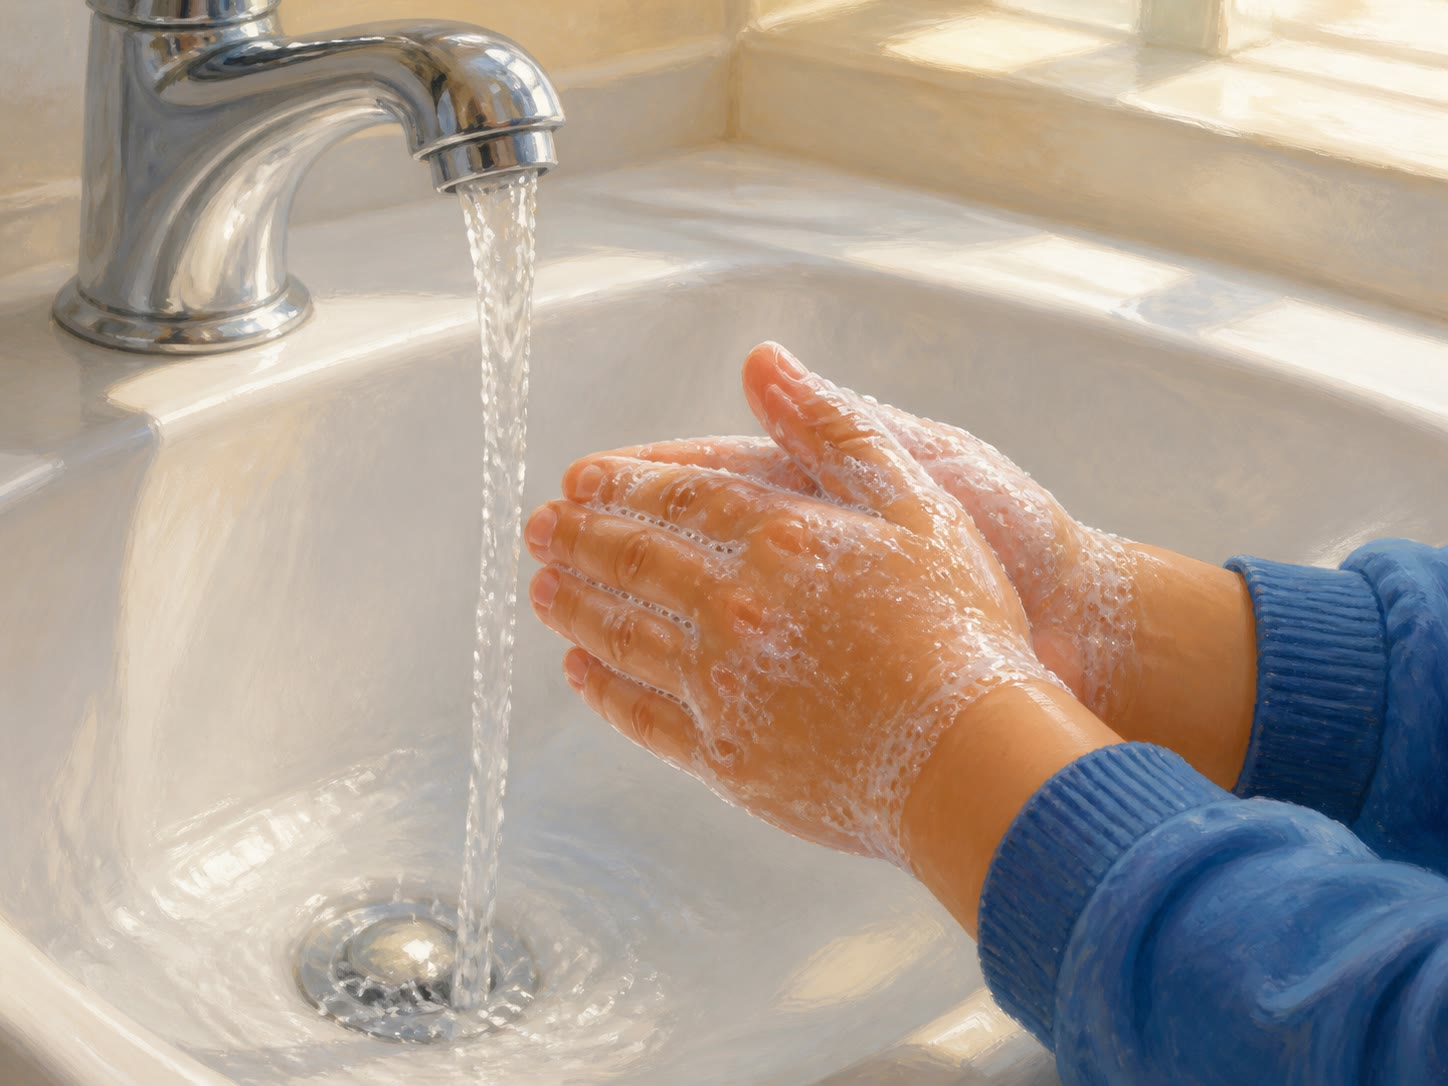
\includegraphics[width=0.58\linewidth]{images/book1/ai/g1-habits-handwashing.jpg}

{\small صابون، وفرك، وماء جارٍ: أبغض أنشودة إلى \omterm{def:g1:healthy-habits:germs}{الجراثيم} تدوم عدًّا
بطيئًا إلى العشرين.}
\end{omfigure}

\begin{example}[تجربة البريق]\label{ex:g1:healthy-habits:glitter}
افرك قليلًا من مسحوق البريق على راحتيك، ثم صافح صديقًا، وافتح
بابًا، والتقط قلمًا: البريق في كل مكان. \omterm{def:g1:healthy-habits:germs}{والجراثيم} تنتقل هكذا
تمامًا، غير أنها غير مرئية. والآن اغسل يديك بالصابون وأنت تعدّ إلى
$20$ --- فيذهب البريق، وتذهب معه \omterm{def:g1:healthy-habits:germs}{الجراثيم}.
\end{example}

\section{أسنان تُحفظ}

\begin{proposition}[لماذا تُنظَّف الأسنان]\label{prop:g1:healthy-habits:teeth}
بعد الأكل تبقى فتات من الطعام على الأسنان. \omterm{def:g1:healthy-habits:germs}{وجراثيم} الفم تتغذى على
هذه البقايا --- وخاصة السكرية منها --- فتحدث في الأسنان ثقوبًا
ببطء، وهي تؤلم. والتنظيف يكنس البقايا قبل أن تولم \omterm{def:g1:healthy-habits:germs}{الجراثيم}.
\end{proposition}
\admitted

\begin{method}[تنظيف أسناني]\label{met:g1:healthy-habits:brush}
\begin{enumerate}
  \item نظّف أسنانك بعد الفطور وقبل \omterm{prop:g1:healthy-habits:needs}{النوم} --- كل يوم؛
  \item ونظّف كل وجه من كل سنّ: الأمام، والخلف، والأعلى حيث تمضغ؛
  \item وخذ وقتك --- نحو مدة أنشودة؛
  \item وبدّل فرشاتك بأخرى جديدة حين تتفرق شعيراتها.
\end{enumerate}
\end{method}

\begin{remark}[الأسنان اللبنية مهمة أيضًا]\label{rem:g1:healthy-habits:babyteeth}
``هذه الأسنان ستسقط على كل حال --- فلم ننظفها؟'' لأن عليها أن
تمضغ لك سنوات بعد، ولأن ثقوبها تؤلم بالقدر نفسه، ولأن أسنان الكبر
تنتظر تحتها منذ الآن وتستحق أن تصل إلى فم نظيف صحيح.
\end{remark}

\section{الأكل والحركة والنوم}

\begin{proposition}[الحاجات اليومية الثلاث]\label{prop:g1:healthy-habits:needs}
يحتاج الجسم النامي كل يوم إلى:
\begin{enumerate}
  \item \emph{غذاء متنوع}\index{غذاء متنوع} --- قليل من كل شيء:
        الخضر والفواكه، والخبز والحبوب، والحليب والجبن، واللحم أو
        السمك أو البيض، والماء للشرب؛ والحلوى بين حين وآخر فحسب؛
  \item \emph{حركة}\index{حركة} --- جري، وتسلق، وركوب دراجة، ولعب
        في الخارج: فالحركة تقوّي العضلات والعظام والقلب؛
  \item \emph{نوم}\index{نوم} --- ففي الليل يستريح الجسم، ويصلح
        نفسه، وينمو؛ والطفل يحتاج إلى ليل طويل، أطول بكثير من ليل
        الكبير.
\end{enumerate}
\end{proposition}
\admitted

\begin{omfigure}
\begin{tikzpicture}
  \draw[thick, omMeth, fill=omMeth!7, rounded corners=6pt]
    (0,0) rectangle (3.6,2.3);
  \draw[thick, omProp, fill=omProp!7, rounded corners=6pt]
    (4.0,0) rectangle (7.6,2.3);
  \draw[thick, omDef, fill=omDef!7, rounded corners=6pt]
    (8.0,0) rectangle (11.6,2.3);
  \node[font=\small\bfseries, omMeth] at (1.8,1.95) {كُلْ متنوعًا};
  \node[font=\small\bfseries, omProp] at (5.8,1.95) {تحرّك};
  \node[font=\small\bfseries, omDef] at (9.8,1.95) {نَمْ};
  \node[font=\small, align=center, text width=3.3cm] at (1.8,0.9)
    {قليل من\\ كل شيء،\\ وماء للشرب};
  \node[font=\small, align=center, text width=3.3cm] at (5.8,0.9)
    {العب في الخارج،\\ واجرِ، وتسلّق،\\ كل يوم};
  \node[font=\small, align=center, text width=3.3cm] at (9.8,0.9)
    {ليل طويل:\\ الجسم يصلح نفسه\\ وينمو};
\end{tikzpicture}

{\small حاجات الجسم النامي اليومية الثلاث. ولا تغني واحدة منها عن
الأخرى.}
\end{omfigure}

\begin{example}[يوم جيد للجسم]\label{ex:g1:healthy-habits:day}
فطور فيه فاكهة؛ ويدان مغسولتان قبل الغداء؛ وأصيل من الجري في
المتنزه؛ وأسنان منظّفة بعد العشاء؛ وإطفاء للأنوار باكرًا مع حكاية.
لا شيء خارق --- وهذا هو المقصود: الصحة تُبنى من أيام عادية كهذا
اليوم.
\end{example}

\begin{remark}[التعب رسالة]\label{rem:g1:healthy-habits:tired}
التثاؤب، ولذع \omterm{def:g1:the-five-senses:sense}{العينين}، والضجر بلا سبب: هذا هو الجسم يقول ``أحتاج
إلى \omterm{prop:g1:healthy-habits:needs}{النوم}''. والإصغاء إليه عادة صحية أيضًا. ودماغ الصباح بعد \omterm{prop:g1:healthy-habits:needs}{نوم}
جيد يتعلم أحسن، ويلعب أحسن، ويضحك أسهل.
\end{remark}

\section{تمارين}

\begin{exercise}[$\star$]\label{exo:g1:healthy-habits:1}
ما \omterm{def:g1:healthy-habits:germs}{الجراثيم}؟ ولماذا قد تحتاج الأيدي التي تبدو نظيفة إلى الغسل؟
\end{exercise}

\begin{exercise}[$\star$]\label{exo:g1:healthy-habits:2}
اذكر ثلاثة أوقات من اليوم يجب فيها غسل اليدين.
\end{exercise}

\begin{exercise}[$\star$]\label{exo:g1:healthy-habits:3}
في \cref{met:g1:healthy-habits:hands}، كم ينبغي أن يدوم الفرك
بالصابون؟ وسمِّ موضعين يسهل نسيانهما.
\end{exercise}

\begin{exercise}[$\star$]\label{exo:g1:healthy-habits:4}
لماذا تصير في الأسنان ثقوب حين لا تُنظَّف؟ احكِ القصة \omterm{def:g1:healthy-habits:germs}{بالجراثيم}
والبقايا.
\end{exercise}

\begin{exercise}[$\star$]\label{exo:g1:healthy-habits:5}
متى ينبغي تنظيف الأسنان؟ وكم ينبغي أن يستغرق؟
\end{exercise}

\begin{exercise}[$\star$]\label{exo:g1:healthy-habits:6}
سمِّ الحاجات اليومية الثلاث في \cref{prop:g1:healthy-habits:needs}،
ومثالًا واحدًا على كل واحدة من يومك أنت.
\end{exercise}

\begin{exercise}[$\star$]\label{exo:g1:healthy-habits:7}
ماذا يفعل الجسم في أثناء \omterm{prop:g1:healthy-habits:needs}{النوم}؟ ومن يحتاج إلى الليل الأطول، الطفل
أم الكبير؟
\end{exercise}

\begin{exercise}[$\star$]\label{exo:g1:healthy-habits:8}
اذكر علامتين على أن الجسم يطلب \omterm{prop:g1:healthy-habits:needs}{النوم}.
\end{exercise}

\begin{exercise}[$\star\star$]\label{exo:g1:healthy-habits:9}
يقول سام: ``أسناني اللبنية ستسقط على كل حال، فتنظيفها لا فائدة
منه.'' أجبه وفق \cref{rem:g1:healthy-habits:babyteeth} --- بسببين
على الأقل.
\end{exercise}

\begin{exercise}[$\star\star$]\label{exo:g1:healthy-habits:10}
في تجربة البريق في \cref{ex:g1:healthy-habits:glitter}، علام يدل
البريق؟ وماذا تبين التجربة عن المصافحة --- وعن الصابون؟
\end{exercise}
